\providecommand{\main}{../..}
\documentclass[\main/thesis.tex]{subfiles}

\begin{document}

\section{Carcinogen Concentration Spatial Distribution}
We consider three different carcinogen spatial distributions (CSD) given by the equations below and shown in Figure \ref{fig:CarcinFunc_FunctionDistributions}:
\begin{align}
    &\text{CSD1: } \frac{1}{2} \left ( \sin\left(\frac{2\pi x}{N}\right) \cos\left(\frac{\pi y}{N}\right) + 1 \right ); \label{eq:CarcinFunc1}\\
    &\text{CSD2: } \text{exp} \left ( -\frac{1}{2} \frac{(x - \mu)^2 + (y - \mu)^2}{\sigma} \right ), \mu = \frac{N}{2} - 1, \sigma = \frac{N}{15}; \label{eq:CarcinFunc2}\\
    &\text{CSD3: } \sum_{i{=}1}^{5} \text{exp} \left ( -\frac{1}{2} \frac{(x - \mu_x^i)^2 + (y - \mu_y^i)^2}{\sigma} \right ), \sigma = \frac{N}{15}, \label{eq:CarcinFunc3}\\
&\mu_x = \{ \frac{N}{2} {-} 1, \frac{N}{4} {-} \sigma {-} 1, N {-} \frac{N}{4} {+} \sigma {-} 1, \frac{N}{4} {-} \sigma {-} 1, N {-} \frac{N}{4} {+} \sigma {-} 1 \}, \nonumber \\
&\mu_y = \{ \frac{N}{2} {-} 1, \frac{N}{4} {-} \sigma {-} 1, N {-} \frac{N}{4} {+} \sigma {-} 1, N {-} \frac{N}{4} {+} \sigma {-} 1, \frac{N}{4} {-} \sigma {-} 1 \}, \nonumber
\end{align}
where $N$ is the domain size, assuming a square domain is used. The carcinogen is present within the domain starting at the initial seed (time-step zero). Since the solution of a diffusion equation and CSD2 are both Gaussian distributions the dynamics and results are comparable. Therefore, we will not discuss the case of using the diffusion equation since it only changes the timing of events relative to CSD2 because it cover a larger region of the domain. Throughout this section we consider CSD2 to be the default spatial distribution, thus other than when comparing between the spatial distributions all the comparisons are against CSD2. 
\begin{figure}[H]
    \centering
    \begin{subfigure}[t]{.25\textwidth}
      \centering
      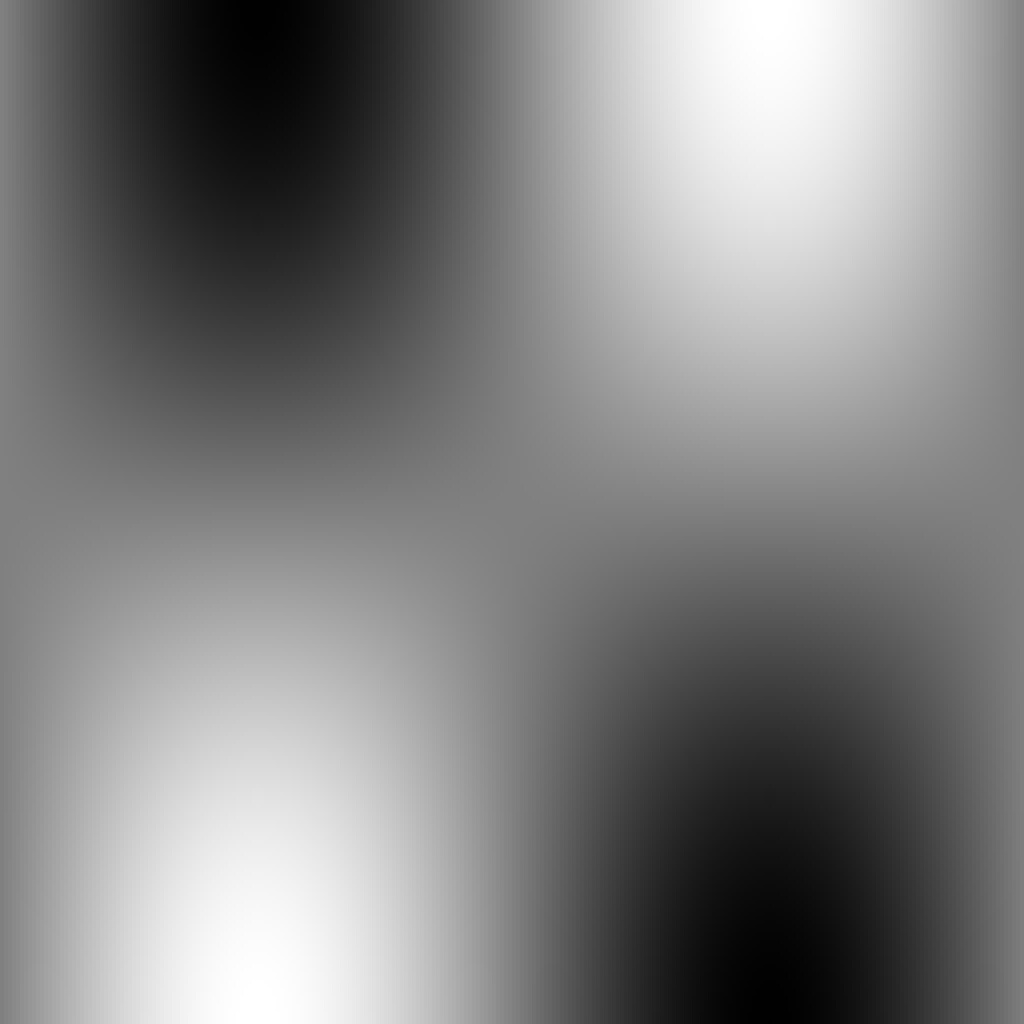
\includegraphics[width=\textwidth]{images/4_CarcinFunc/Fig1/Func1.jpeg}
      \caption{CSD1}
      \label{fig:CarcinFunc_Func1Distribution}
    \end{subfigure}
    \begin{subfigure}[t]{.25\textwidth}
      \centering
      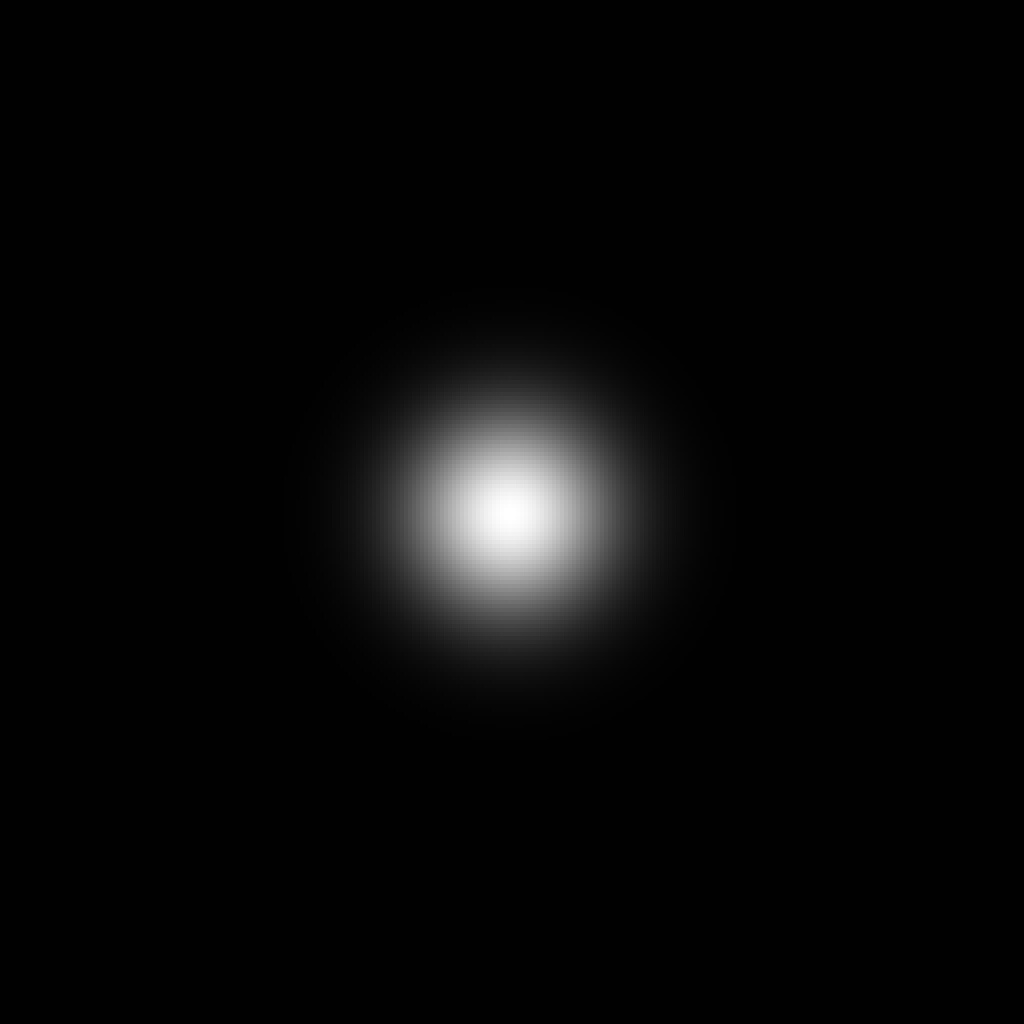
\includegraphics[width=\textwidth]{images/4_CarcinFunc/Fig1/Func2.jpeg}
      \caption{CSD2}
      \label{fig:CarcinFunc_Func2Distribution}
    \end{subfigure}
    \begin{subfigure}[t]{.25\textwidth}
      \centering
      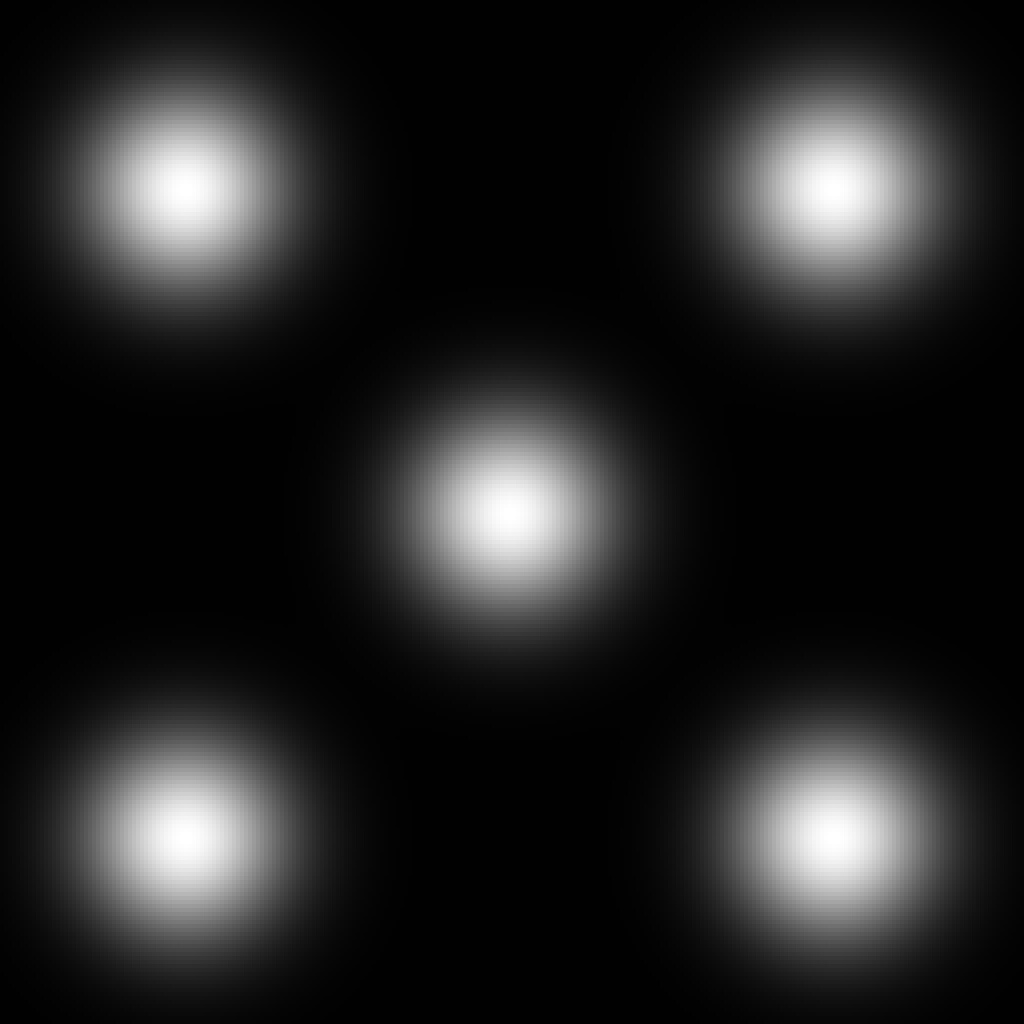
\includegraphics[width=\textwidth]{images/4_CarcinFunc/Fig1/Func3.jpeg}
      \caption{CSD3}
      \label{fig:CarcinFunc_Func3Distribution}
    \end{subfigure}
    \caption{This figure shows a visual representation of each of the carcinogen spatial distributions within a 256x256 domain. In the figures we show (a) carcinogen spatial distribution 1 (CSD1), (b) CSD2, and (c) CSD3.}
    \label{fig:CarcinFunc_FunctionDistributions}
\end{figure}

In Figure \ref{fig:CarcinFunc_numState} we present the time evolution of the fraction of cells in the different cell classes. In (a) we use CSD1, in (b) CSD2, and in (c) CSD3. Videos of the scenarios CSD2 and CSD3 are provided at \href{https://youtu.be/eKxsrSoDiKs}{Hybrid Cellular Automata of Field Cancerization Example 1} and \href{https://youtu.be/Gtf6MoxXCkM}{Hybrid Cellular Automata of Field Cancerization Example 2}, which each contain three simultaneous videos including from left to right the carcinogen spatial distribution, the CA grid, and a visualization that shows the top twenty cell lineages. We observe in all graphs that the fraction of normal tissue (brown, blue) decreases to be replaced by the cancer field (mutated cells: green, yellow, and purple). The cancer field is later replaced by the tumour cells (red). The fraction of mutated stem cells decreases along with the mutated cells, while the fraction of cancer stem cells increases as the cancer increases. The field starts to form at around 10 months as it correlates to four genes being positively mutated in at least one cell. Note that a spike in empty cells occurs soon after the beginning of field formation due to the fact that there are insufficient MNSC to create TAC which rejuvenate the MNTC. CSD1 results in the most expeditious development of a field and tumours, because the function covers most of the domain and has the highest average intensity within the domain. CSD3 is the next to develop a field and tumours, it is ahead of CSD2 because CSD3 has five Gaussian distributions to CSD2's one, thus events have a higher probability of occurring due to the carcinogen(s) covering more of the domain. Figure \ref{fig:CarcinFunc_numState} shows us that the field develops at approximately the same rate for CSD1 and CSD3. When CSD2 is used the MNTCs and MNSCs do not reach as high of a fraction of the domain, compared to CSD1 and CSD3, before the tumour cells take over. 
\begin{figure}[H]
    \centering
    \begin{subfigure}[t]{.6\textwidth}
      \centering
      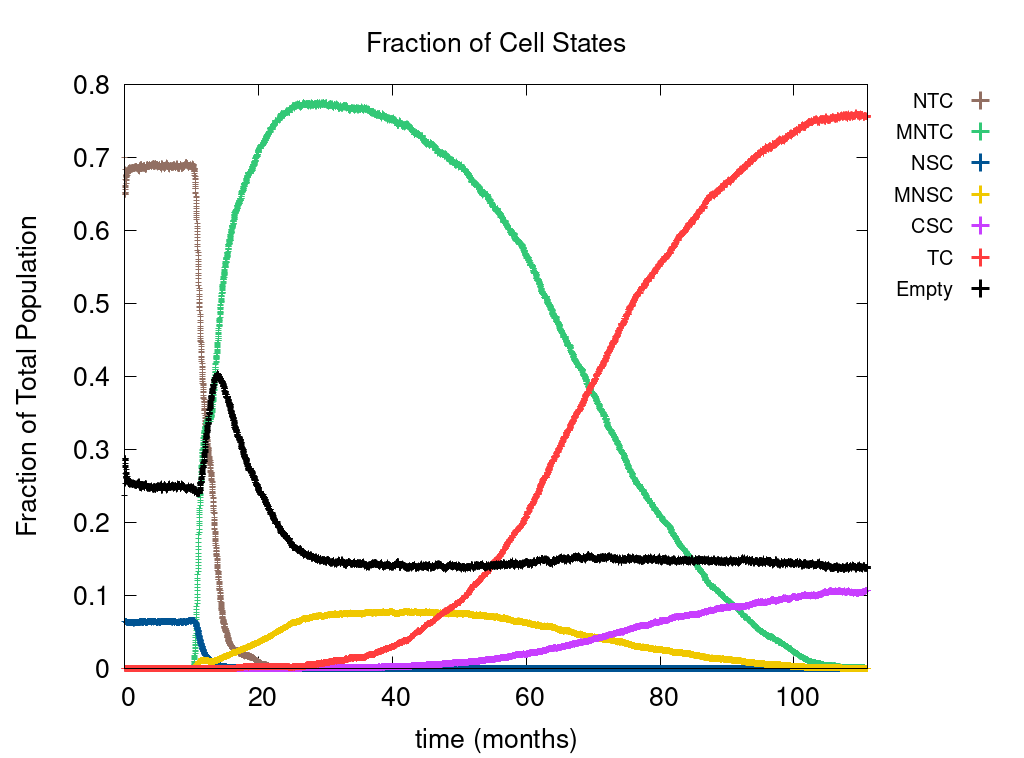
\includegraphics[width=\textwidth]{images/4_CarcinFunc/Fig2/numState_all_Func1.png}
      \caption{CSD1}
      \label{fig:CarcinFunc_numState_Func1}
    \end{subfigure}
    \begin{subfigure}[t]{.6\textwidth}
      \centering
      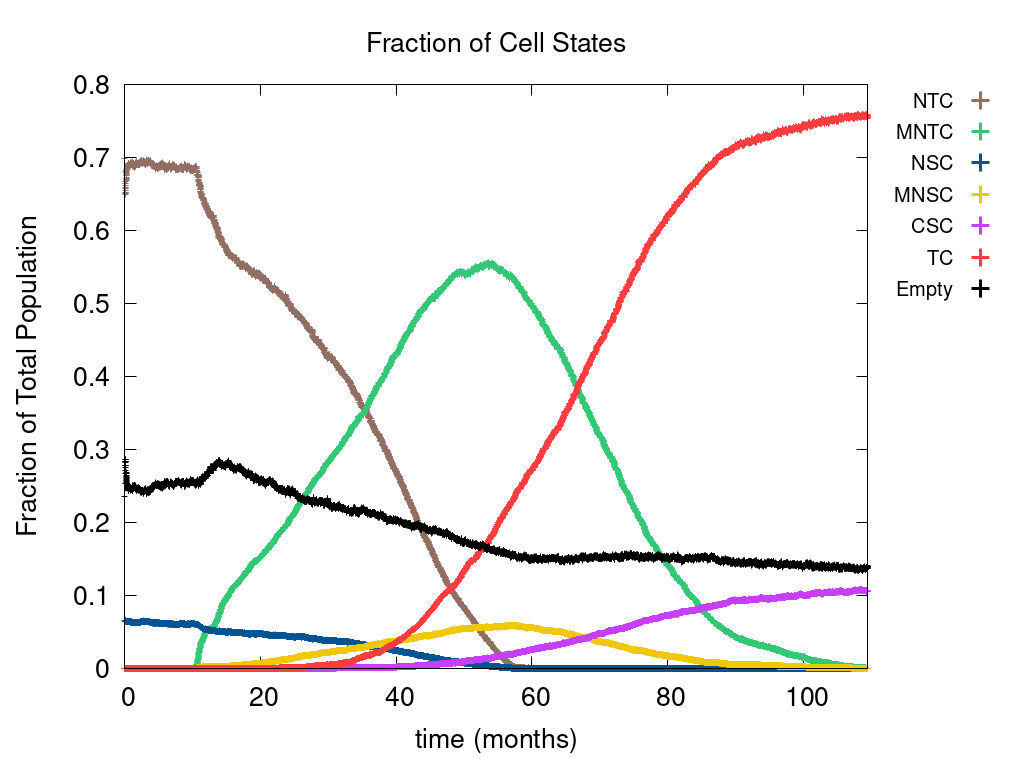
\includegraphics[width=\textwidth]{images/4_CarcinFunc/Fig2/numState_all_Func2.png}
      \caption{CSD2}
      \label{fig:CarcinFunc_numState_Func2}
    \end{subfigure}
    \begin{subfigure}[t]{.6\textwidth}
      \centering
      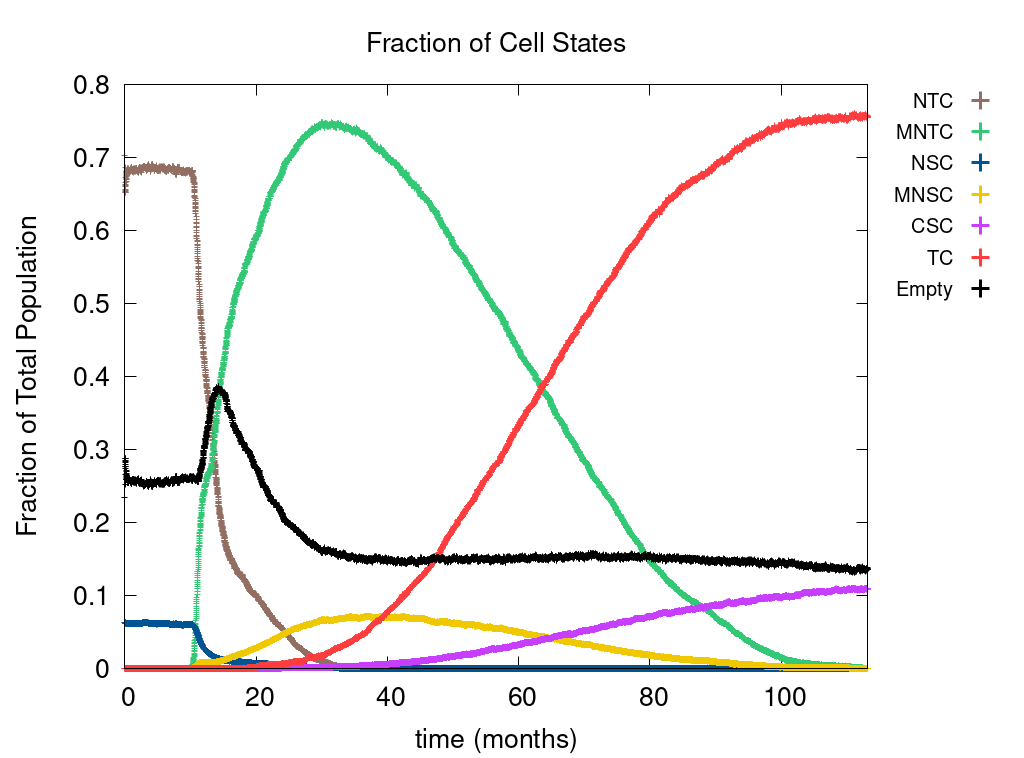
\includegraphics[width=\textwidth]{images/4_CarcinFunc/Fig2/numState_all_Func3.png}
      \caption{CSD3}
      \label{fig:CarcinFunc_numState_Func3}
    \end{subfigure}
    \caption{In figures (a),(b),(c) we show the time course of the fraction of cells in the different cell classes NTC, MNTC, NSC, MNSC, CSC, TC, empty. In (a) we consider carcinogen spatial distribution 1 (CSD1), in (b) CSD2, and in (c) CSD3. Parameters are as follows: grid size 256x256 and both carcinogens activated.}
    \label{fig:CarcinFunc_numState}
\end{figure}

In Figure \ref{fig:CarcinFunc_geneExpr} we show the time evolution of the average gene expression for each of the ten genes. In (a) we show CSD1, in (b) we show CSD2, and in (c) we show CSD3. We see that no matter what carcinogen spatial distribution is used, all the genes become positively mutated. Figure \ref{fig:CarcinFunc_geneExpr} shows that the mutation rate for CSD1 and CSD3 is linear, whereas for CSD2 it is initially exponential before becoming linear; less cells would be mutated and as a result averaging would affect the curve. 
\begin{figure}[H]
    \centering
    \begin{subfigure}[t]{.6\textwidth}
      \centering
      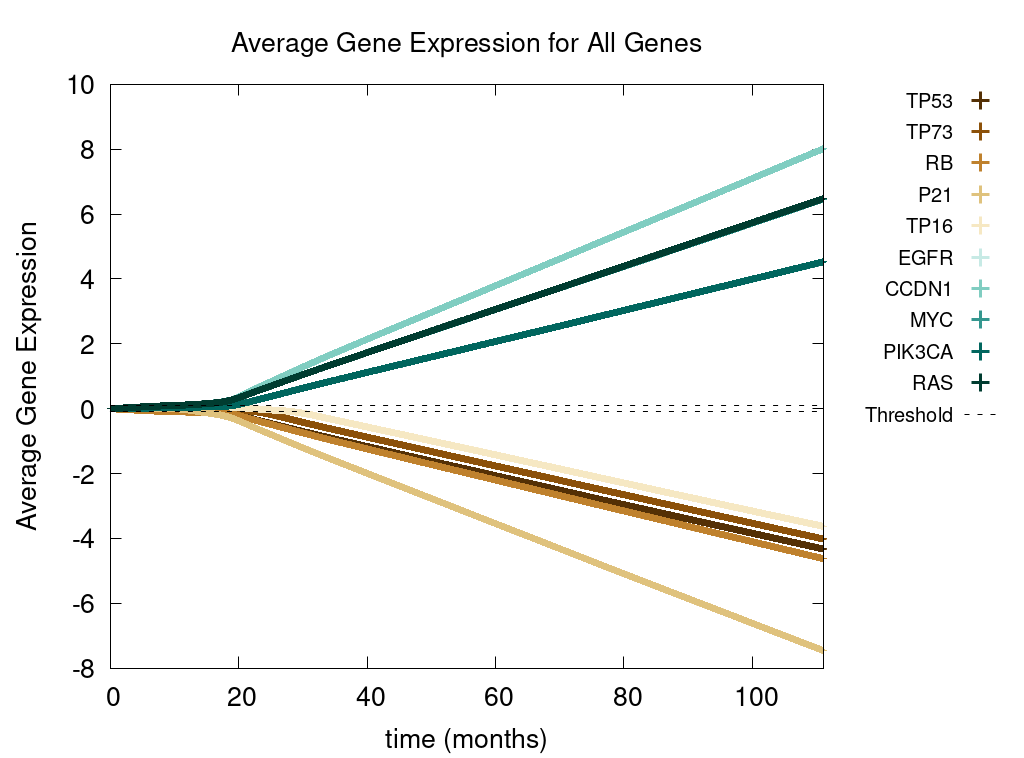
\includegraphics[width=\textwidth]{images/4_CarcinFunc/Fig3/geneExprAll_all_Func1.png}
      \caption{CSD1}
      \label{fig:CarcinFunc_geneExpr_Func1}
    \end{subfigure}
    \begin{subfigure}[t]{.6\textwidth}
      \centering
      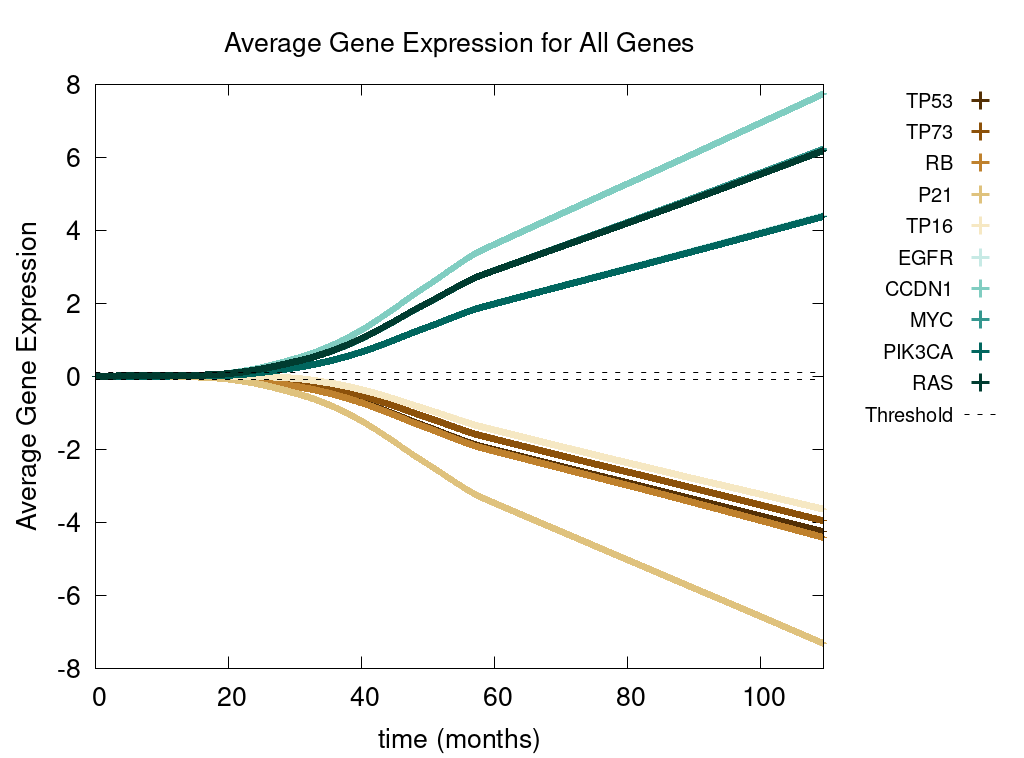
\includegraphics[width=\textwidth]{images/4_CarcinFunc/Fig3/geneExprAll_all_Func2.png}
      \caption{CSD2}
      \label{fig:CarcinFunc_geneExpr_Func2}
    \end{subfigure}
    \begin{subfigure}[t]{.6\textwidth}
      \centering
      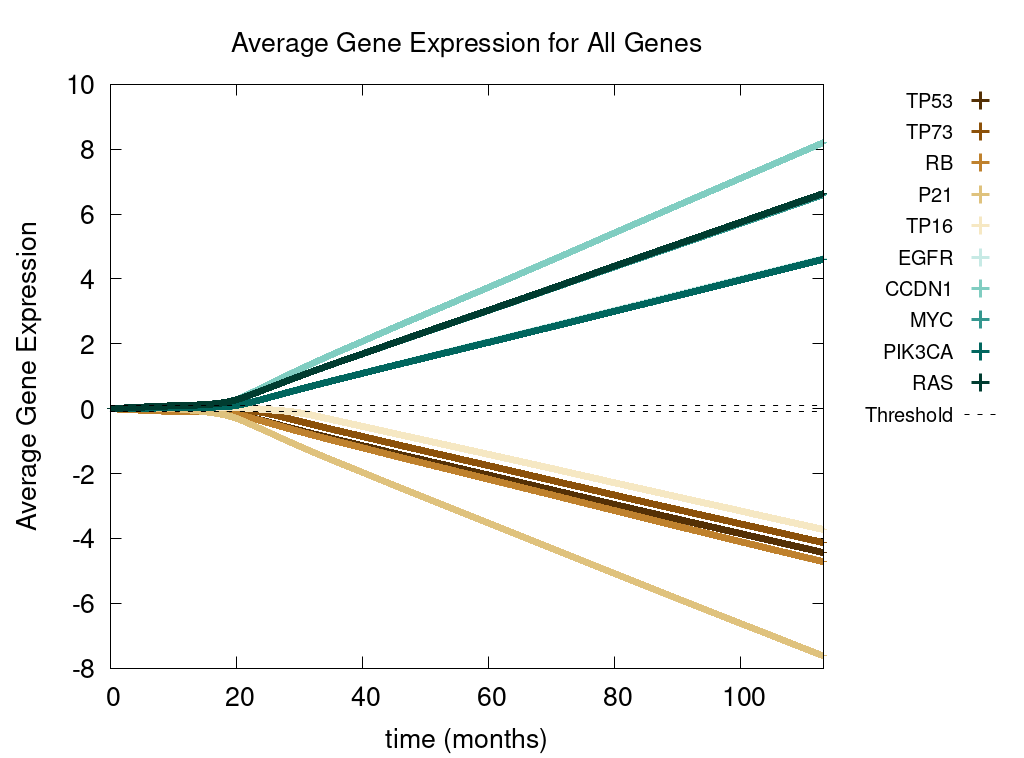
\includegraphics[width=\textwidth]{images/4_CarcinFunc/Fig3/geneExprAll_all_Func3.png}
      \caption{CSD3}
      \label{fig:CarcinFunc_geneExpr_Func3}
    \end{subfigure}
    \caption{In figures (a),(b),(c) we show the time course of the average gene expression for each of the ten genes. In the plots we consider (a) carcinogen spatial distribution 1 (CSD1), (b) CSD2, and (c) CSD3. Parameters are as follows: grid size 256x256 and both carcinogens activated.}
    \label{fig:CarcinFunc_geneExpr}
\end{figure}

In Figure \ref{fig:CarcinFunc_numPheno} we show the time evolution of the fraction of cells that underwent each of the phenotypic actions, namely proliferation (purple), apoptosis (blue), quiescence (moved, green), and differentiation (orange). In (a) we consider CSD1, in (b) CSD2, and in (c) CSD3. For all the carcinogen spatial distributions we see that as the cancer field develops, proliferation increases, apoptosis decreases, and cell movement and differentiation remain approximately constant. When the field begins forming there is a spike in differentiation caused by more empty cells being available. Figure \ref{fig:CarcinFunc_numPheno} shows that all the spatial distributions have similar phenotypic evolution. Cell movement spikes less for CSD2, as compared to CSD1 and CSD3, due to the smaller coverage of the domain. Proliferation declines more for CSD1 and CSD3, as compared to CSD2, during the early stages of the field, due to competition for empty cells from cell movement caused by higher probability of quiescence. 
\begin{figure}[H]
    \centering
    \begin{subfigure}[t]{.6\textwidth}
      \centering
      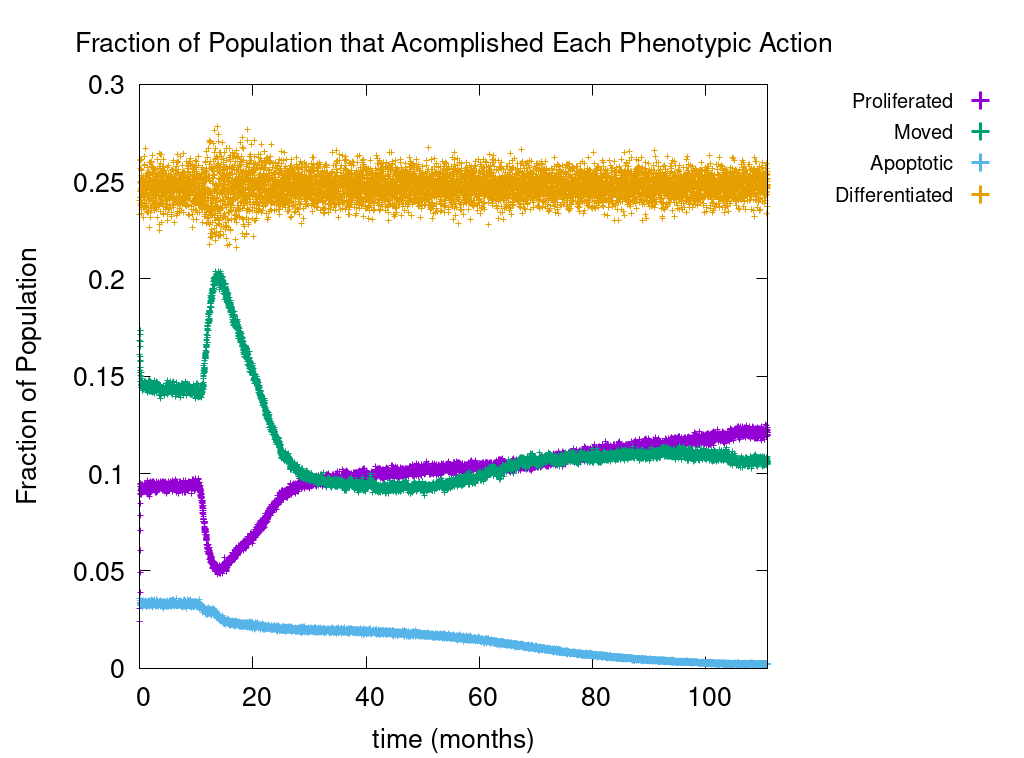
\includegraphics[width=\textwidth]{images/4_CarcinFunc/Fig4/numPheno_all_Func1.png}
      \caption{CSD1}
      \label{fig:CarcinFunc_numPheno_Func1}
    \end{subfigure}
    \begin{subfigure}[t]{.6\textwidth}
      \centering
      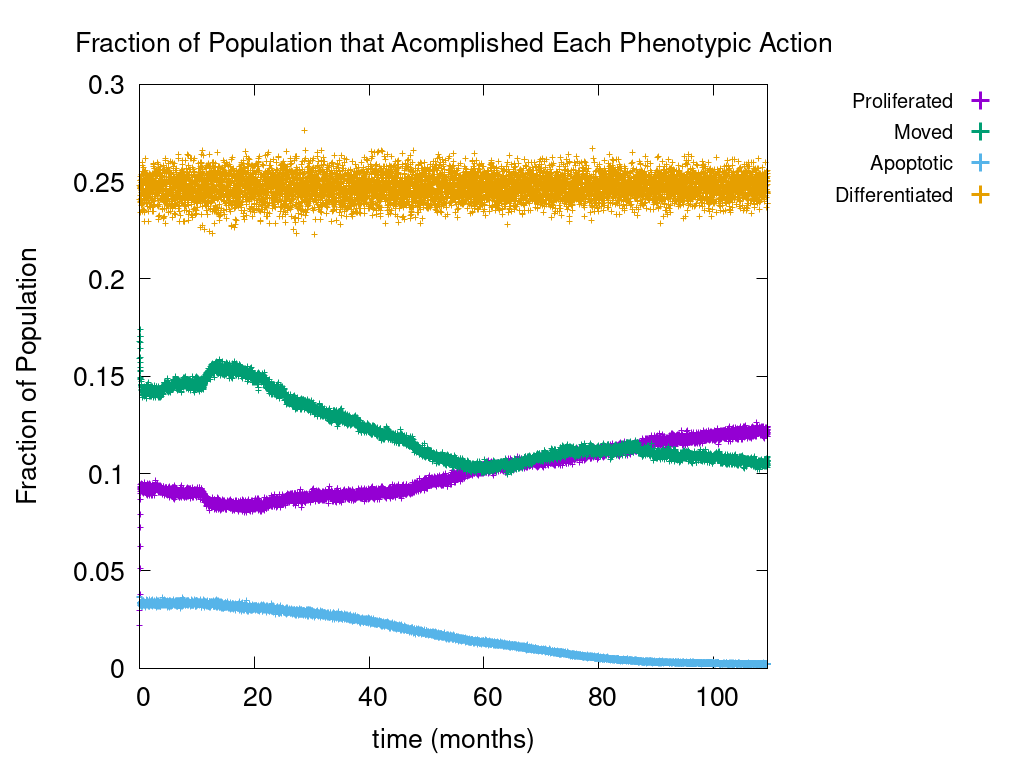
\includegraphics[width=\textwidth]{images/4_CarcinFunc/Fig4/numPheno_all_Func2.png}
      \caption{CSD2}
      \label{fig:CarcinFunc_numPheno_Func2}
    \end{subfigure}
    \begin{subfigure}[t]{.6\textwidth}
      \centering
      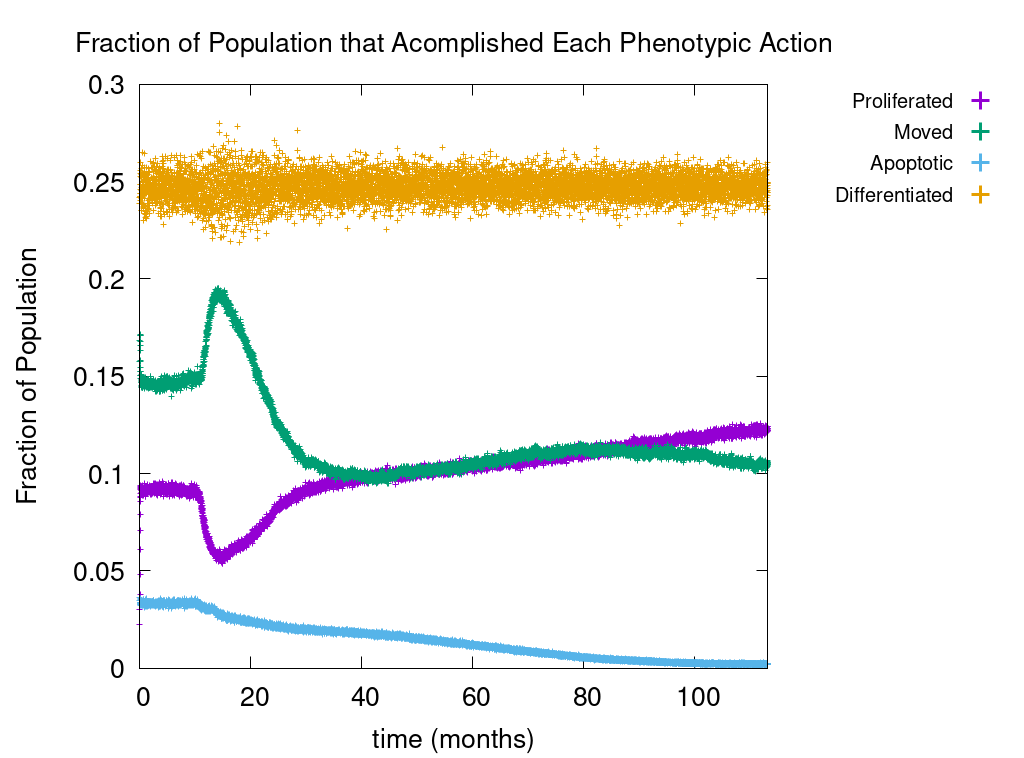
\includegraphics[width=\textwidth]{images/4_CarcinFunc/Fig4/numPheno_all_Func3.png}
      \caption{CSD3}
      \label{fig:CarcinFunc_numPheno_Func3}
    \end{subfigure}
    \caption{In figures (a),(b),(c) we show the time course of the fraction of cells that underwent each of the phenotypic actions, namely proliferation, apoptosis, quiescence (moved), and differentiation. In the plots we consider (a) carcinogen spatial distribution 1 (CSD1), (b) CSD2, and (c) CSD3. Parameters are as follows: grid size 256x256 and both carcinogens activated.}
    \label{fig:CarcinFunc_numPheno}
\end{figure}

In Figure \ref{fig:CarcinFunc_Characteristics} we compare various characteristics of the cancer field and cancer development between the carcinogen spatial distributions (CSDs). In the plots, we show (a) the time evolution of the fraction of positively mutated genes, (b) the time evolution of the average cell fitness, (c) the time evolution of the log of the number of cell lineages, and (d) the time evolution of the fraction of cells that are part of the tumour mass(es).
Figure \ref{fig:CarcinFunc_numPosMut} shows us that all the genes become positively mutated for the three distributions, however, it takes CSD2 longer than the rest. Figure \ref{fig:CarcinFunc_fitness} reveals to us that the fitness increases at a similar rate for the three distributions, with CSD2 being more delayed in the increase and having a lower fitness overall. Figure \ref{fig:CarcinFunc_numLineages} indicates that the number of cell lineages decreases, however, at the period 40-60 months CSD2 decreases rapidly until it stabilizes and continues decreasing at the same rate as the other two. This occurs because the point at which the first TC is formed the field in CSD2 is significantly smaller, thus the TCs overtake the field more quickly than the other two cases, as demonstrated in Figure \ref{fig:CarcinFunc_numState}. Finally, Figure \ref{fig:CarcinFunc_TumourMassGrowthCurve} shows us that the tumour growth rate curve has a similar shape for all the distributions, with CSD1 requiring the most time to fill the domain, followed by CSD3, and CSD2 requiring the least amount of time. This phenomenon is explained by less competition occurring between lineages for CSD2. More carcinogen in the domain leads to faster development of the field.
\begin{figure}[H]
    \centering
    \begin{subfigure}[t]{.49\textwidth}
      \centering
      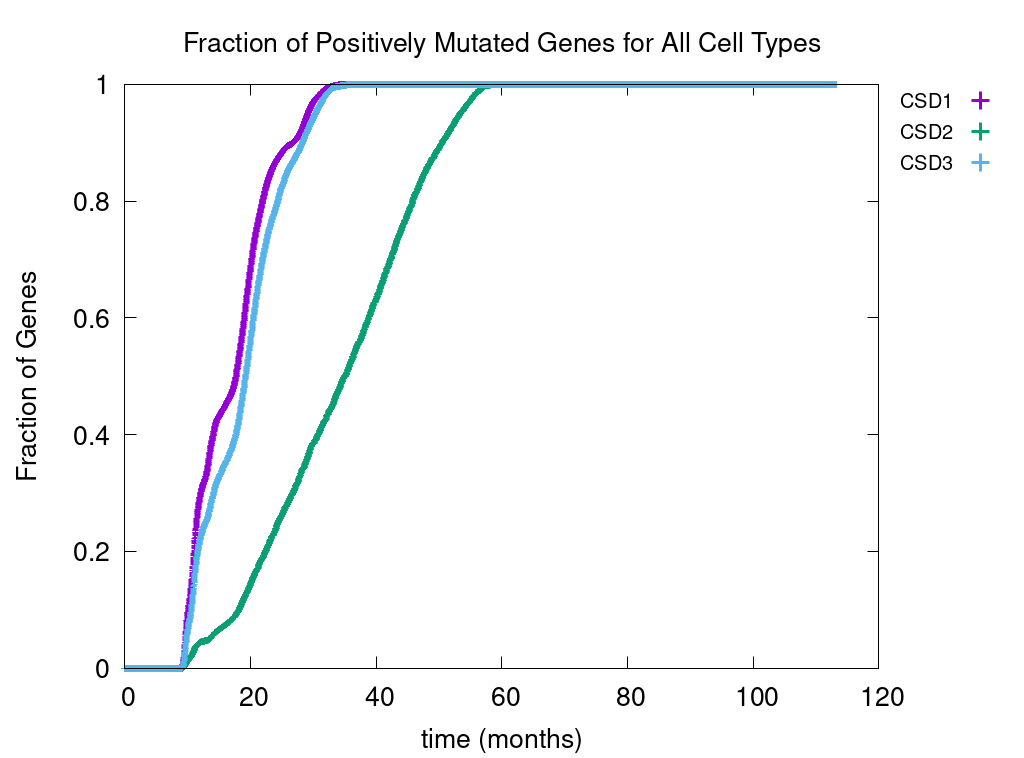
\includegraphics[width=\textwidth]{images/4_CarcinFunc/Fig5/numPosMut_CarcinFuncs.png}
      \caption{Positively mutated gene fraction}
      \label{fig:CarcinFunc_numPosMut}
    \end{subfigure}
    \begin{subfigure}[t]{.49\textwidth}
      \centering
      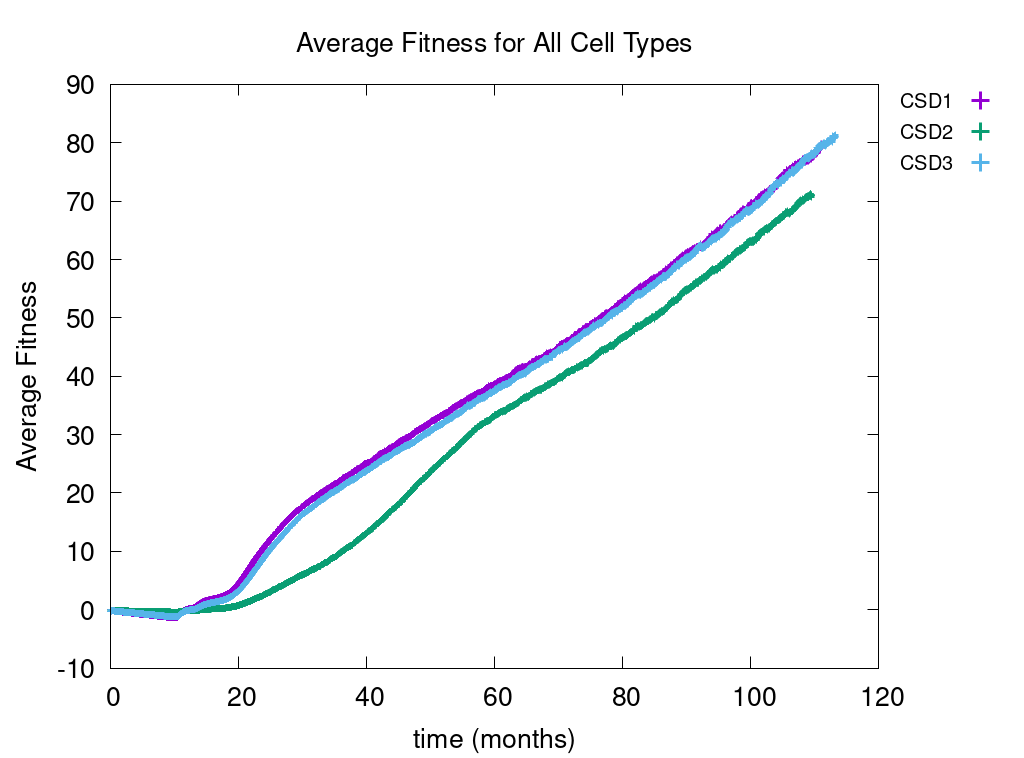
\includegraphics[width=\textwidth]{images/4_CarcinFunc/Fig5/fitness_CarcinFuncs.png}
      \caption{Average cell fitness}
      \label{fig:CarcinFunc_fitness}
    \end{subfigure}
    \begin{subfigure}[t]{.49\textwidth}
      \centering
      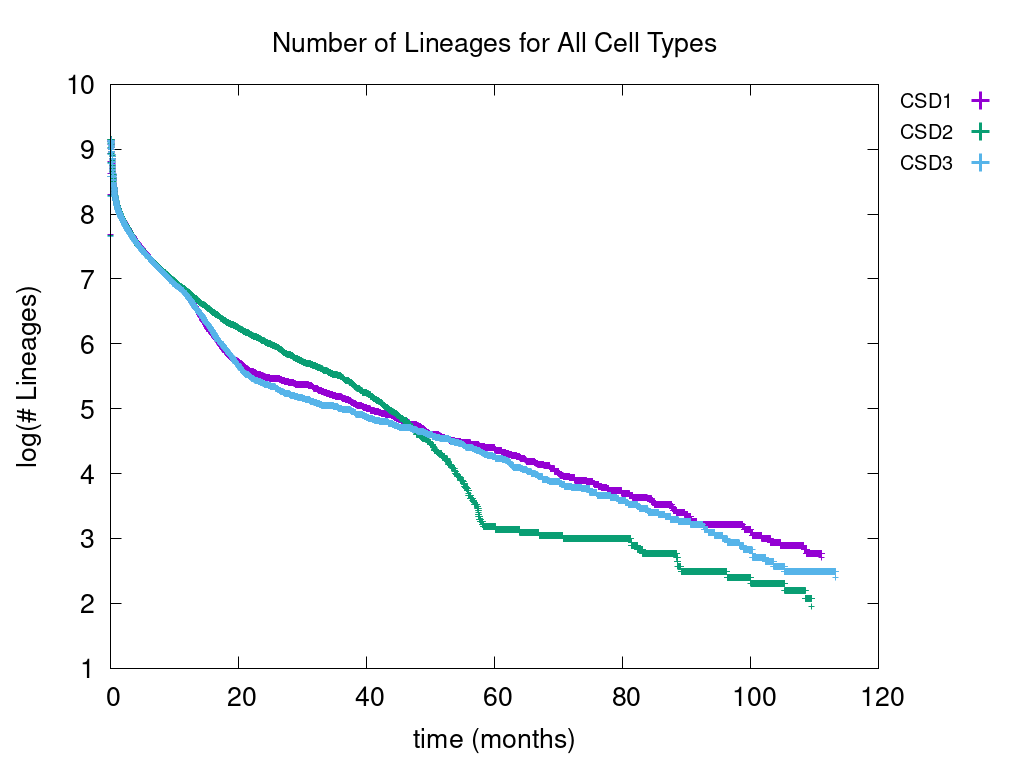
\includegraphics[width=\textwidth]{images/4_CarcinFunc/Fig5/numLineages_CarcinFuncs.png}
      \caption{Number of cell lineages}
      \label{fig:CarcinFunc_numLineages}
    \end{subfigure}
    \begin{subfigure}[t]{.49\textwidth}
      \centering
      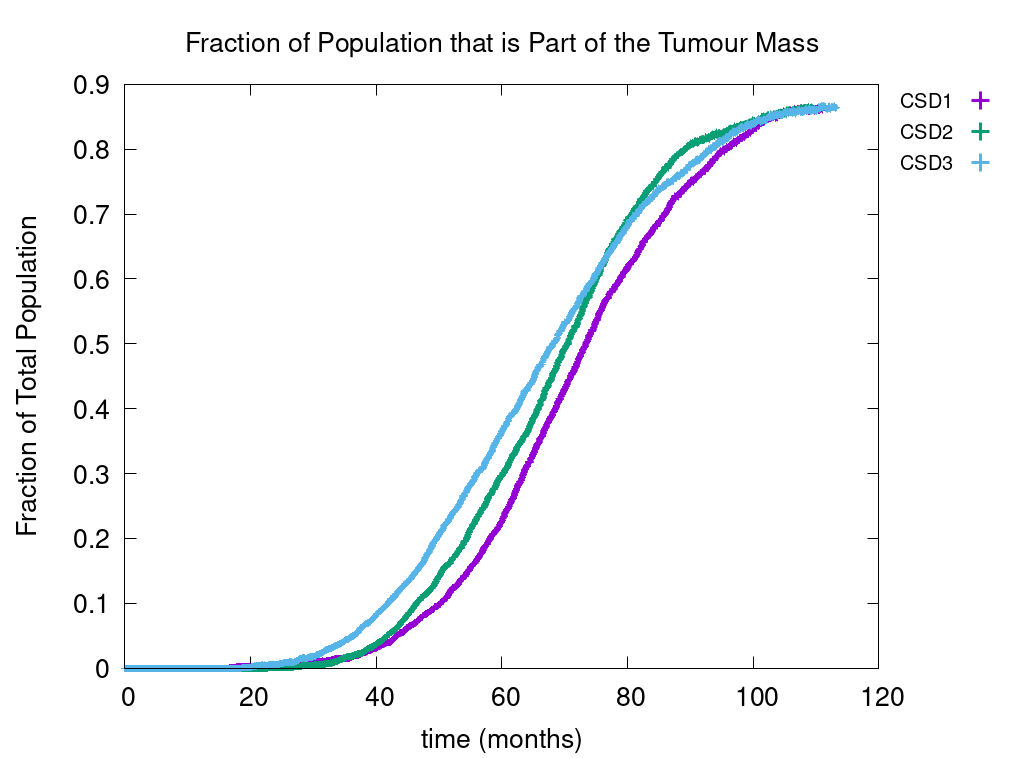
\includegraphics[width=\textwidth]{images/4_CarcinFunc/Fig5/numCSCAndTC_CarcinFuncs.png}
      \caption{Tumour growth rate}
      \label{fig:CarcinFunc_TumourMassGrowthCurve}
    \end{subfigure}
    \caption{In this figure we compare various characteristics of the cancer field and cancer development between the carcinogen spatial distributions (CSD). In the plots we show (a) the time course of the fraction of positively mutated genes, (b) the time course of the average cell fitness, (c) the time course of the log of the number of cell lineages, and (d) the time course of the fraction of cells that are part of the tumour mass(es). Parameters are as follows: grid size 256x256 and both carcinogens activated.}
    \label{fig:CarcinFunc_Characteristics}
\end{figure}

\subsection{Single Carcinogen}
In Figure \ref{fig:CarcinFunc_numState_Carcins} we present the time evolution of the fraction of cells in the different cell classes. In Figure \ref{fig:CarcinFunc_geneExpr_Carcins} we present the time evolution of the average gene expression for each gene. For both figures in (a) we use ethanol and in (b) nicotine. We see that for ethanol (alcohol) the dynamic is very similar to the equilibrium case, except the genes are mutated slightly. Alcohol alone does not cause a field to develop due to the carcinogen causing the majority of the genes to mutate away from cancer, as shown in Figures \ref{fig:CarcinFunc_numState_Carcin0} and \ref{fig:CarcinFunc_geneExpr_Carcin0}. This is in accordance with the biology that states alcohol alone rarely causes oral cancer. Nicotine alone does cause a field to develop because, unlike alcohol, the genes are positively influenced towards cancer, as is evidenced by Figures \ref{fig:CarcinFunc_numState_Carcin1} and \ref{fig:CarcinFunc_geneExpr_Carcin1}. This again agrees with the actual effects of nicotine on the body, as smoking is a major cause of oral and lung cancers. 
\begin{figure}[H]
    \centering
    \begin{subfigure}[t]{.6\textwidth}
      \centering
      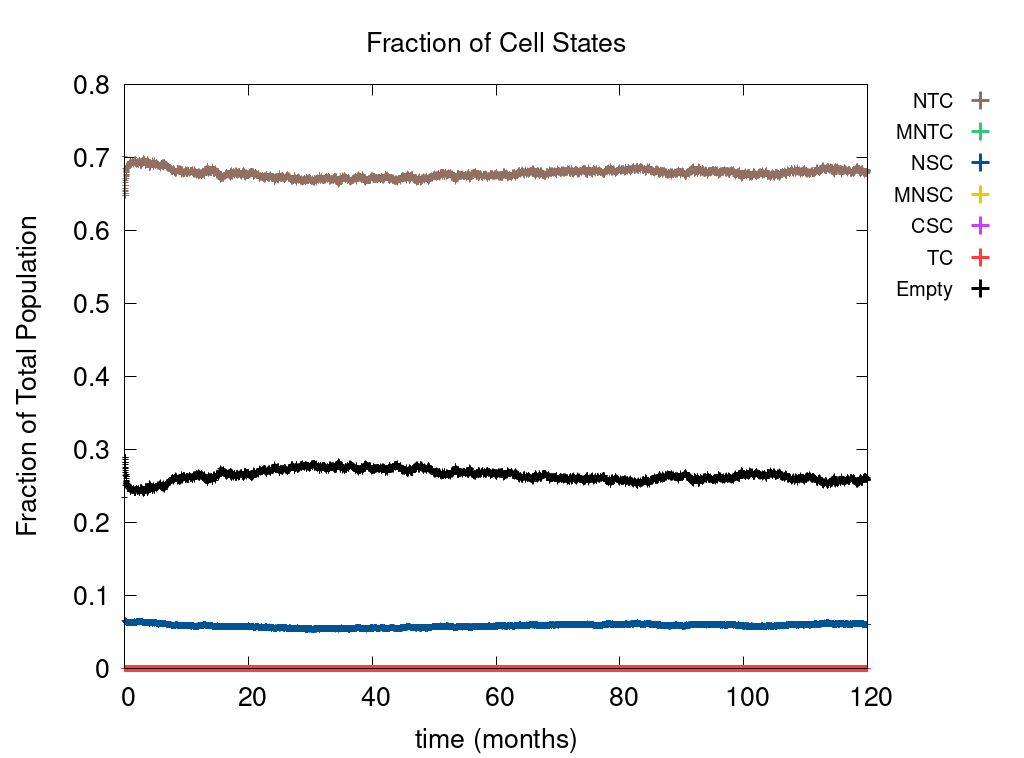
\includegraphics[width=\textwidth]{images/4_CarcinFunc/Fig6/numState_all_Carcin0.png}
      \caption{Ethanol}
      \label{fig:CarcinFunc_numState_Carcin0}
    \end{subfigure}
    \begin{subfigure}[t]{.6\textwidth}
      \centering
      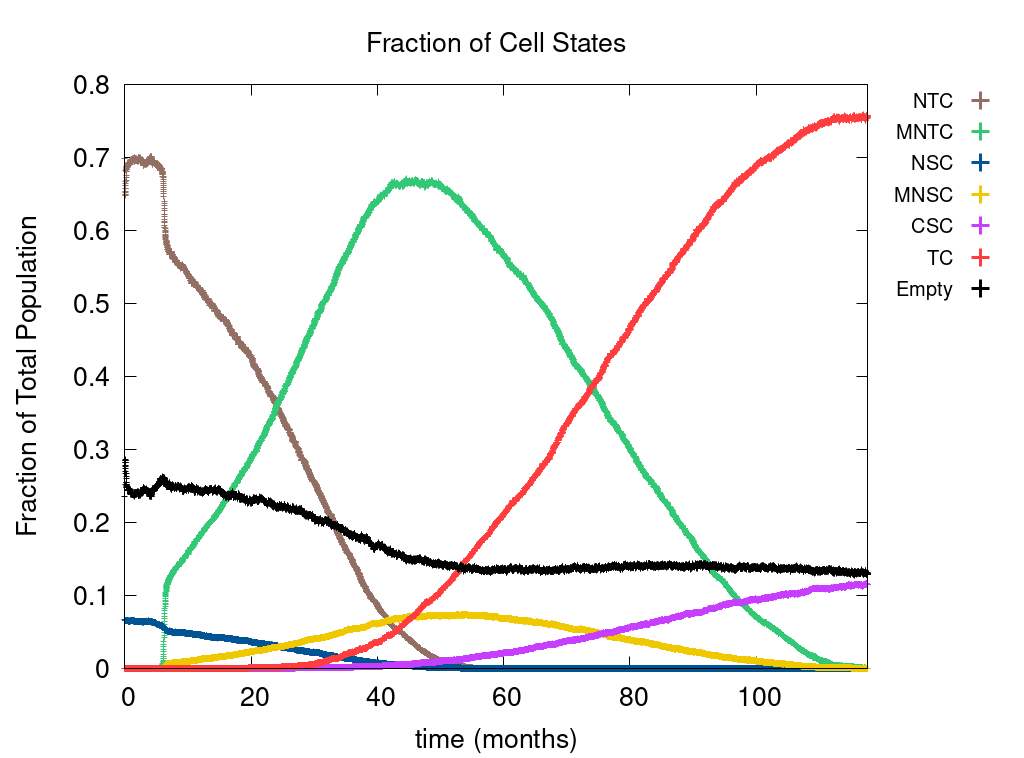
\includegraphics[width=\textwidth]{images/4_CarcinFunc/Fig6/numState_all_Carcin1.png}
      \caption{Nicotine}
      \label{fig:CarcinFunc_numState_Carcin1}
    \end{subfigure}
    \caption{In figures (a),(b) we show the time course of the fraction of cells in the different cell classes NTC, MNTC, NSC, MNSC, CSC, TC, empty. In the plots we consider (a) ethanol and (b) nicotine. Parameters are as follows: grid size 256x256 and carcinogen spatial distribution 2.}
    \label{fig:CarcinFunc_numState_Carcins}
\end{figure}

\begin{figure}[H]
    \centering
    \begin{subfigure}[t]{.6\textwidth}
      \centering
      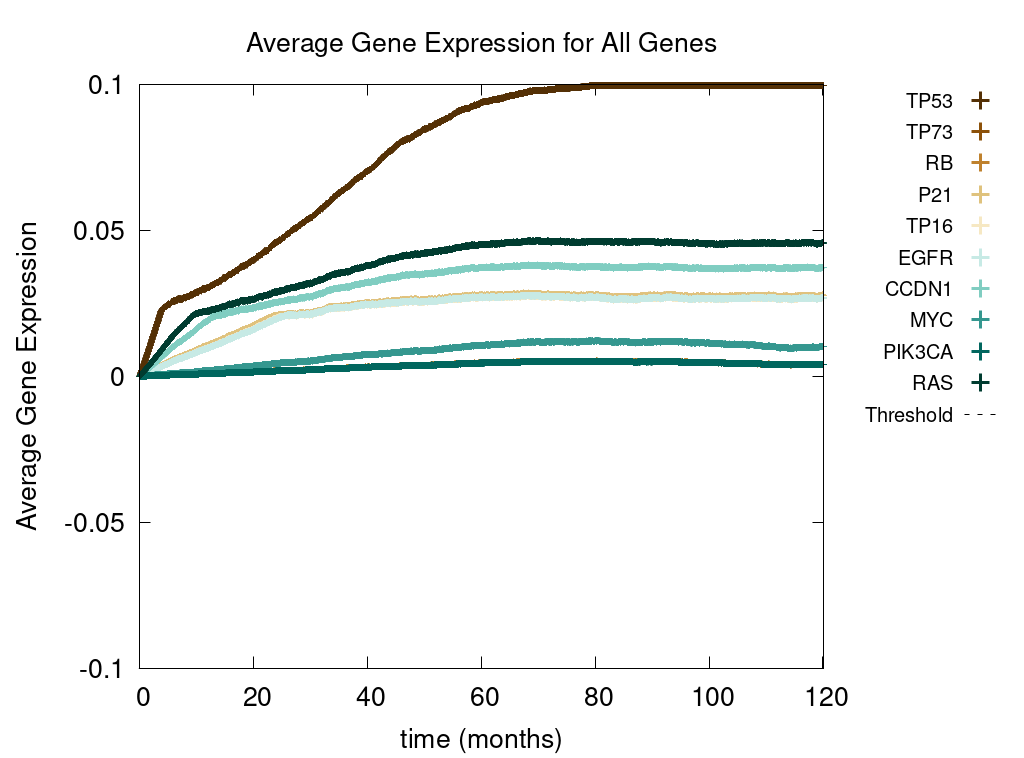
\includegraphics[width=\textwidth]{images/4_CarcinFunc/Fig7/geneExprAll_all_Carcin0.png}
      \caption{Ethanol}
      \label{fig:CarcinFunc_geneExpr_Carcin0}
    \end{subfigure}
    \begin{subfigure}[t]{.6\textwidth}
      \centering
      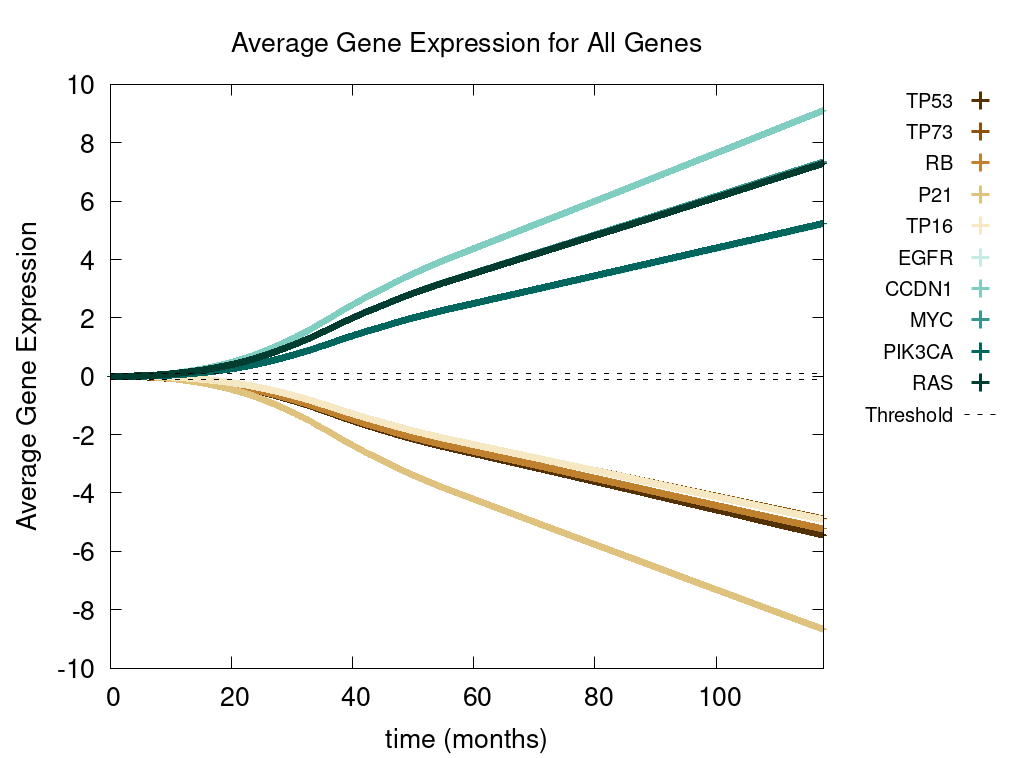
\includegraphics[width=\textwidth]{images/4_CarcinFunc/Fig7/geneExprAll_all_Carcin1.png}
      \caption{Nicotine}
      \label{fig:CarcinFunc_geneExpr_Carcin1}
    \end{subfigure}
    \caption{In figures (a),(b) we show the time course of the average gene expression for each of the ten genes. In the plots we consider (a) ethanol and (b) nicotine. Parameters are as follows: grid size 256x256 and carcinogen spatial distribution 2.}
    \label{fig:CarcinFunc_geneExpr_Carcins}
\end{figure}

If we had considered a different tissue such as the liver and/or included more genes that are positively mutated by alcohol, then it is probable that alcohol would cause a field and, eventually, cancer. In particular, alcohol would likely develop cancer in the liver as it has a high mutagenic effect on the liver \cite{Bagnardi,Grewal,Petrick}.

\subsection{All Carcinogens}
When both carcinogens are included, a cancer field and tumour always develop. Tumour development is faster when both carcinogens are active compared to nicotine alone, as is demonstrated by comparing Figures \ref{fig:CarcinFunc_numState_Func2} and \ref{fig:CarcinFunc_numState_Carcin1}. Analyzing the figures, we can conclude that although the field initiates first in the nicotine case and becomes larger, the tumour grows at a faster rate in the case that both carcinogens are active. This agrees with the clinical data, which alludes to drinking and smoking in combination increasing the chances of cancer forming relative to one of them alone \cite{cancer.net_2021}. Further it is known that alcohol in combination with smoking increases the chances of developing cancer because the alcohol weakens the cells, which allows the tobacco to be more mutagenic \cite{Weinberg}. This combined impact of the carcinogens is what causes the field to be smaller than the nicotine alone. In the case of nicotine being the sole carcinogen, the field initiates faster since it does not have to fight against the mutagenic effects of alcohol. The tumour growth rate is quicker in the two-carcinogen case because there is more carcinogen within the domain, thus more gene mutations will accrue.

\subsection{Cyclic Carcinogenic Onslaught}
We analyze various realistic scenarios where the carcinogen(s) are removed from the domain in a cyclic fashion. For all the simulations we use a grid size of 256x256 and CSD2 (equation \ref{eq:CarcinFunc2}). In Figure \ref{fig:CarcinFunc_numState_CyclicCarcin} we show the time evolution of the fraction of cells in the different cell classes. In the plots, we have the case of (a) smoking every day and drinking on weekends, (b) smoking on weekends, and (c) smoking on weekdays. A video of the scenario of smoking on weekends is provided at \href{https://youtu.be/4CTrhoddFOw}{Hybrid Cellular Automata of Field Cancerization Example 3}, which contains three simultaneous videos including from left to right the carcinogen spatial distribution, the CA grid, and a visualization that shows the top twenty cell lineages.  We can see the field starts to develop earlier in cases (a) and (c) relative to case (b), as evidenced by the MNTC (green) and MNSC (yellow) curves. Additionally, in case (a) the field reaches a larger size, relative to cases (b) and (c), as is established by the MNTC and MNSC curves. The first TC forms earlier in cases (a) and (c) compared to case (b). The rate of tumour growth is slightly faster in (a) and (c) as compared to (b), although (c) is slightly faster than (a).
\begin{figure}[H]
    \centering
    \begin{subfigure}[t]{.6\textwidth}
      \centering
      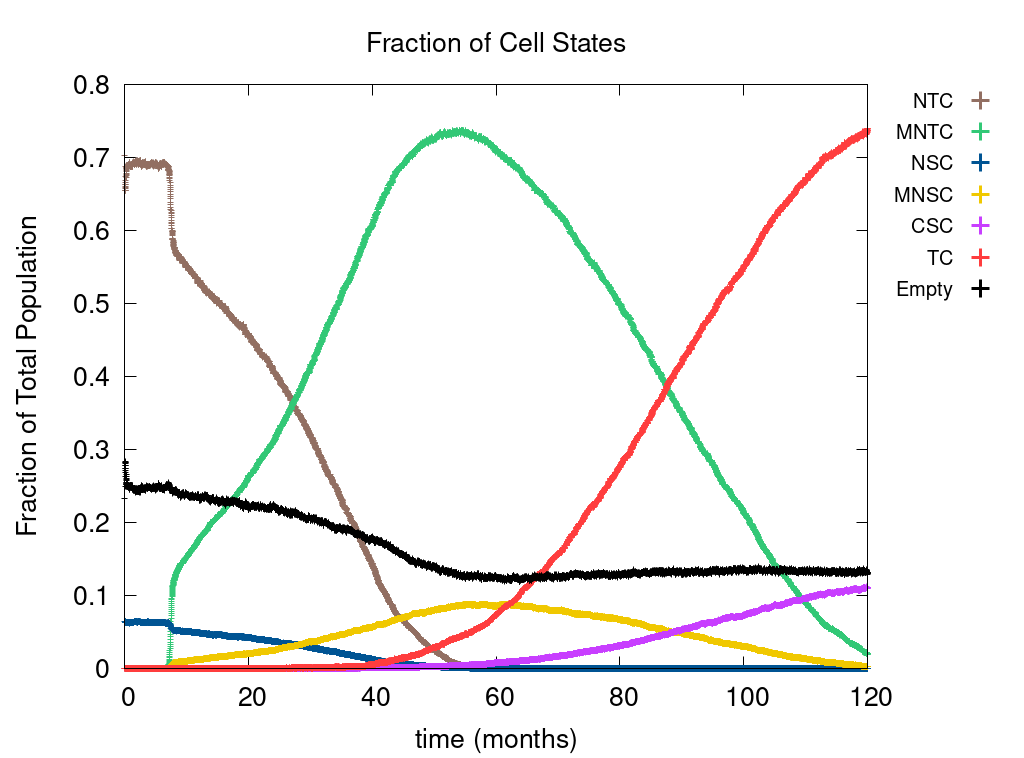
\includegraphics[width=\textwidth]{images/4_CarcinFunc/Fig8/numState_all_DrinkEveryday_SmokeWeekends.png}
      \caption{Smoke every day and drink on weekends}
      \label{fig:CarcinFunc_numState_DrinkEveryday_SmokeWeekends}
    \end{subfigure}
    \begin{subfigure}[t]{.6\textwidth}
      \centering
      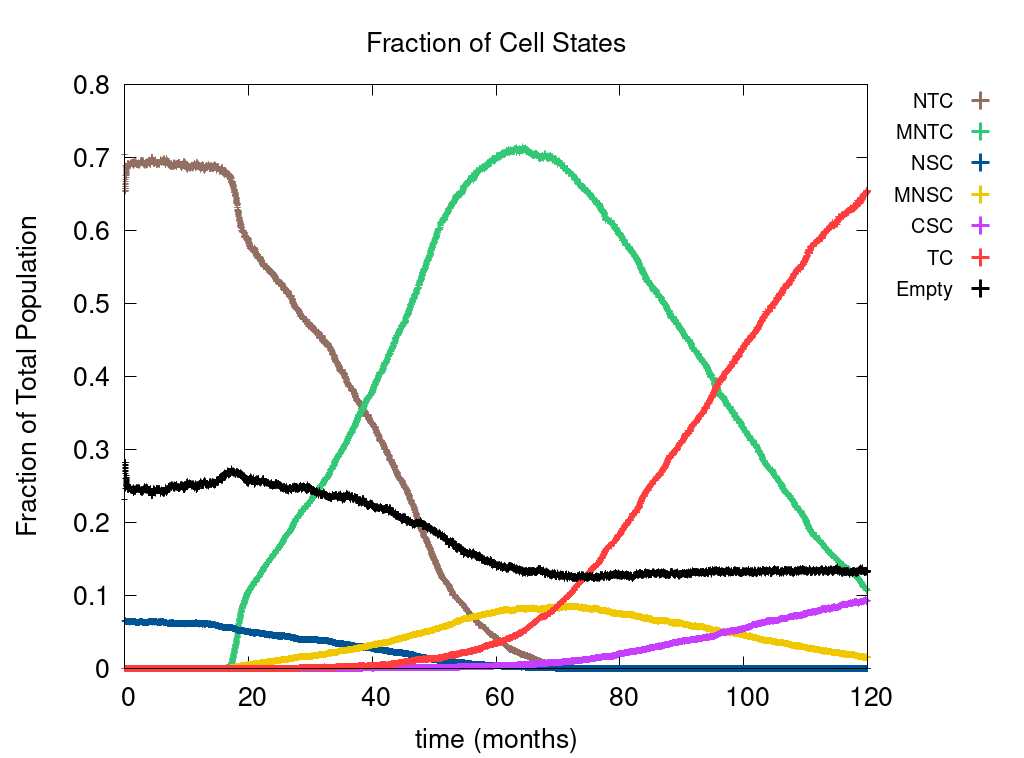
\includegraphics[width=\textwidth]{images/4_CarcinFunc/Fig8/numState_all_SmokeWeekends.png}
      \caption{Smoke on weekends}
      \label{fig:CarcinFunc_numState_SmokeWeekends}
    \end{subfigure}
    \begin{subfigure}[t]{.6\textwidth}
      \centering
      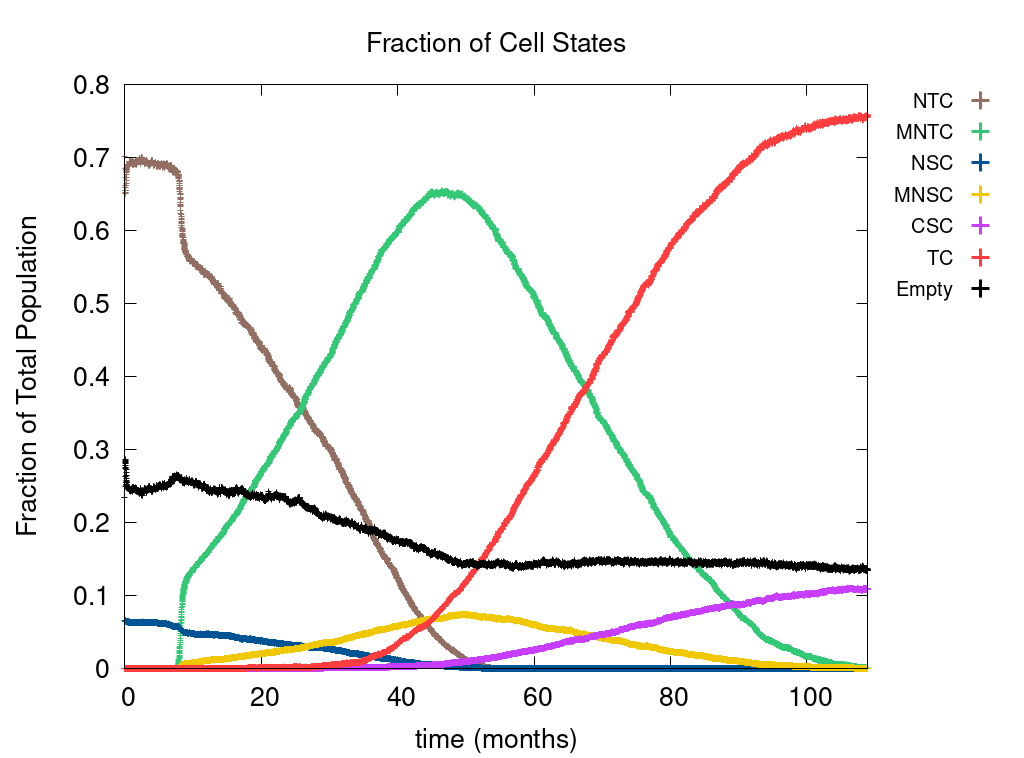
\includegraphics[width=\textwidth]{images/4_CarcinFunc/Fig8/numState_all_SmokeWeekdays.png}
      \caption{Smoke on weekdays}
      \label{fig:CarcinFunc_numState_SmokeWeekdays}
    \end{subfigure}
    \caption{In figures (a),(b),(c) we show the time course of the fraction of cells in the different cell classes NTC, MNTC, NSC, MNSC, CSC, TC, empty. In the plots we show the case of (a) smoking every day and drinking on weekends, (b) smoking on weekends, and (c) smoking on weekdays. Parameters are as follows: grid size 256x256 and carcinogen spatial distribution 2.}
    \label{fig:CarcinFunc_numState_CyclicCarcin}
\end{figure}

As noted above, the development of the field in Figure \ref{fig:CarcinFunc_numState_SmokeWeekends} in which the only carcinogen is nicotine and smoking occurs on weekends only, is vastly delayed and develops much less rapidly as compared to the other two figures. This is to be expected since in this case there is a large reduction in the carcinogenic onslaught due in part to the lack of alcohol consumption and to the large reduction of nicotine. Further, we note that it takes the body up-to four days after smoking stops for it to be cleared of nicotine \cite{Benowitz}, thus nicotine will still continue to mutate the genes during the days of non-smoking.

When comparing these three scenarios it was noted that onset of cancer is slower and grows at a slightly lower rate in the scenario of smoking every day and drinking on weekends versus the scenario in which smoking occurs on weekdays only. This contradicts what was observed in the comparison of Figures \ref{fig:CarcinFunc_numState_Func2} (smoking and drinking every day) and \ref{fig:CarcinFunc_numState_Carcin1} (smoking every day) in which the combined impact of the two carcinogens caused more rapid cancer growth. Thus, it is shown that the negative impacts of the alcohol in combination with nicotine are negated somewhat when alcohol is only consumed on the weekend. In fact it would appear in this case that this small amount of alcohol fights against the mutations being caused by the nicotine.

Comparing the difference of this impact of the amount of alcohol consumption is also illustrated by comparing Figure \ref{fig:CarcinFunc_numState_DrinkEveryday_SmokeWeekends} with \ref{fig:CarcinFunc_numState_Func2} in which the alcohol consumption occurred every day along with smoking. The field develops faster when less alcohol is consumed due to the lack of alcohol during the week which would otherwise be fighting the positive mutations caused by the nicotine. The onset of cancer and the rate of cancer growth when drinking every day with smoking is significantly greater than when only drinking on the weekends. Further, confirming the impact of cancer growth when two carcinogens are introduced and the impact of the onslaught of carcinogens.

The final case is the impact of the quantity of nicotine alone, thus we compare Figure \ref{fig:CarcinFunc_numState_SmokeWeekdays} (smoking on weekdays) versus Figure \ref{fig:CarcinFunc_numState_Carcin1} (smoking every day). The dynamics between the two are near identical illustrating that if a heavy smoker only ceases smoking for two days per week, it is not a sufficient reduction in onslaught to impact the results. This is due to the fact that in the model once carcinogen onslaught has caused some positively mutated genes to occur, then those genes will continue to mutate throughout the two day period.  

\end{document}